\section{Mathematical Framework}

\subsection{Problem Definition}

Consider a set of \(P\) variables, where the \(p\)-th variable contains \(L_p\) observations as \(\boldsymbol{x} = \{(t_l^{(p)}, x_l^{(p)})\}_{l=1, p=1}^{L_p, P} \), being \(x_l^{(p)} \in \mathbb{R}\) the corresponding observation at time \(t_l^{(p)} \in \mathbb{R}\). A graph representation of that structure with \(P=3\) is plotted in \cref{fig:input_sample_structure}. Each \(\boldsymbol{x}\) has its own target variable \(\boldsymbol{y} \in \mathbb{R}^D \), leading to a collection of \(N\) input-output i.i.d. pairs denoted as \(\mathcal{D} = \{\boldsymbol{x}_n, \boldsymbol{y}_n\}_{n=1}^N\) = \(\{\boldsymbol{X}, \boldsymbol{Y}\}\) called training set. The task is to generalize the map from each input \(\boldsymbol{x}\) to its corresponding target output \(\boldsymbol{y}\) in a stochastic fashion.




\begin{figure}[ht]
	\centering
	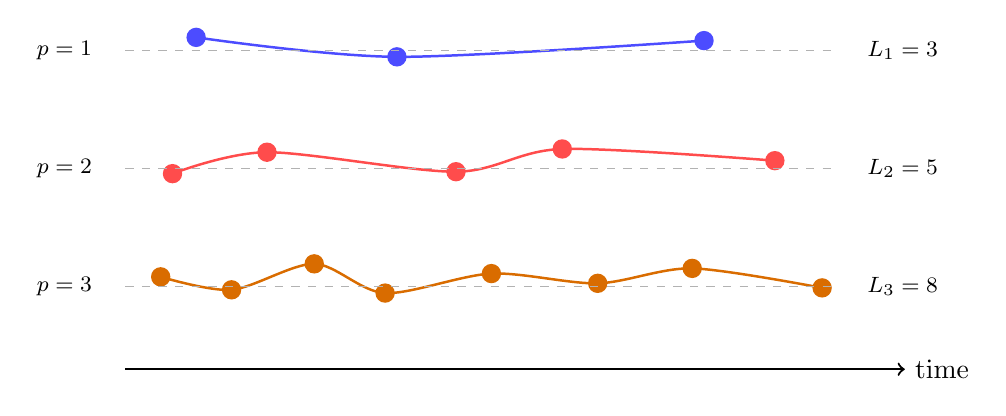
\begin{tikzpicture}[x=1.5cm,y=1.5cm]
	%		\usetikzlibrary{calc}
	
	% --- parámetros ---
	\newcommand{\Tmin}{0}
	\newcommand{\Tmax}{6}
	\newcommand{\ValScale}{0.55}
	
	% --- listas (t / x) ---
	\def\sOne{0.6/ 0.20, 2.3/-0.10, 4.9/ 0.15}                                   % L1=3
	\def\sTwo{0.4/-0.08, 1.2/ 0.25, 2.8/-0.05, 3.7/0.30, 5.5/0.12}               % L2=5
	\def\sThr{0.3/ 0.15, 0.9/-0.05, 1.6/0.35, 2.2/-0.10, 3.1/0.20,               % L3=8
		4.0/ 0.05, 4.8/0.28, 5.9/-0.02}
	
	% offsets verticales
	\newcommand{\yOne}{2.0}
	\newcommand{\yTwo}{1.0}
	\newcommand{\yThr}{0.0}
	
	% estilos
	\tikzset{
		base/.style = {black!30, dashed},
		line1/.style = {line width=0.9pt, blue!70},
		line2/.style = {line width=0.9pt, red!70},
		line3/.style = {line width=0.9pt, orange!85!black},
		dot/.style   = {circle, minimum size=3.2pt, inner sep=0pt},
	}
	
	% macro para dibujar una serie
	\newcommand{\DrawSeries}[4]{% #1=color, #2=y0, #3=lista, #4=Lp
		\def\coords{}%
		\foreach \t/\x in #3 {%
			\pgfmathsetmacro{\yy}{#2 + \ValScale*(\x)}%
			\xdef\coords{\coords (\t,\yy)}%
		}%
		\draw[#1] plot[smooth] coordinates {\coords};
		\foreach \t/\x in #3 {%
			\pgfmathsetmacro{\yy}{#2 + \ValScale*(\x)}%
			\fill[#1] (\t,\yy) circle (3.5pt);
		}%
		% línea base
		\draw[base] (\Tmin,#2) -- (\Tmax,#2);
		% etiquetas p y L
		\node[anchor=east,font=\footnotesize] at (\Tmin-0.2,#2) {$p=#4$};
		\node[anchor=west,font=\footnotesize] at (\Tmax+0.2,#2) {$L_{#4}=\ifnum#4=1 3\else\ifnum#4=2 5\else 8\fi\fi$};
	}
	
	% dibujar las tres series con sus etiquetas
	\DrawSeries{line1}{\yOne}{\sOne}{1}
	\DrawSeries{line2}{\yTwo}{\sTwo}{2}
	\DrawSeries{line3}{\yThr}{\sThr}{3}
	
	% eje de tiempo
	\draw[->, thick] (\Tmin,-0.7) -- (\Tmax+0.6,-0.7) node[anchor=west]{time};
	
\end{tikzpicture}
	\caption{Structure of input samples. Each dot represent a pair \((t_l^{(p)}, x_l^{(p)})\).}
	\label{fig:input_sample_structure}
\end{figure}

\subsection{Likelihood Model}

For this propose, consider a likelihood functions that rule the generation of recorded targets \(\boldsymbol{Y}\) from inputs \(\boldsymbol{X}\) through some set of parameters \(\boldsymbol{\theta} \subseteq \mathbb{R}^J\) 

\begin{equation}\label{eq:likelihood_funciton}
	p\left(\boldsymbol{Y} \mid \boldsymbol{\theta}(\boldsymbol{X})\right) = \prod_{n=1}^N p\left(\boldsymbol{y}_n \mid \boldsymbol{\theta}(\boldsymbol{x}_n)\right). 
\end{equation}

Each element of \( \boldsymbol{\theta}(\boldsymbol{x}) \), denoted as \( \theta_{j}(\boldsymbol{x}) \), could be restricted to some subset of \( \mathbb{R} \). To handle that, we model \( \theta_{j}(\boldsymbol{x}) = h_{j}(f_{j}(\boldsymbol{x})) \) as a transformation of an unrestricted latent variable \( f_{j}(\boldsymbol{x}) \) via a link function \( h_{j} \). Our task boils down to finding the latent vector function \(\boldsymbol{f}(\boldsymbol{x}) = [f_1(\boldsymbol{x}), \cdots, f_J(\boldsymbol{x})]^\top \in \mathbb{R}^J\).